\documentclass{article}
\usepackage{float}
\usepackage{pgfplots}
\pgfplotsset{compat=newest}
\pgfplotsset{plot coordinates/math parser=false}
\usepackage{gnuplot-lua-tikz}

\begin{document}

  \begin{figure}
    \newlength\figureheight
    \newlength\figurewidth
    \setlength\figureheight{0.15\textheight}
    \setlength\figurewidth{0.5\textwidth}
    % This file was created by matplotlib v0.1.0.
% Copyright (c) 2010--2014, Nico Schlömer <nico.schloemer@gmail.com>
% All rights reserved.
% 
% The lastest updates can be retrieved from
% 
% https://github.com/nschloe/matplotlib2tikz
% 
% where you can also submit bug reports and leavecomments.
% 
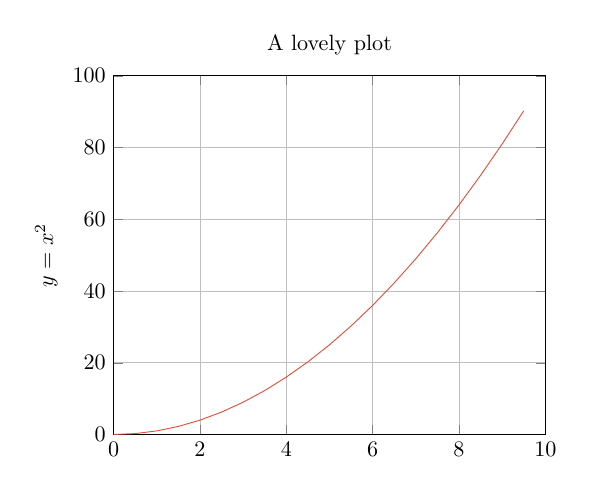
\begin{tikzpicture}[scale=0.8]

\definecolor{color0}{rgb}{0.886274509803922,0.290196078431373,0.2}

\begin{axis}[
title={A lovely plot},
ylabel={$y=x^2$},
xmin=0, xmax=10,
ymin=0, ymax=100,
xmajorgrids,
ymajorgrids
]
\addplot [color0]
coordinates {
(0,0)
(0.5,0.25)
(1,1)
(1.5,2.25)
(2,4)
(2.5,6.25)
(3,9)
(3.5,12.25)
(4,16)
(4.5,20.25)
(5,25)
(5.5,30.25)
(6,36)
(6.5,42.25)
(7,49)
(7.5,56.25)
(8,64)
(8.5,72.25)
(9,81)
(9.5,90.25)

};
\path [draw=white, fill opacity=0] (axis cs:13,0)--(axis cs:13,0);

\path [draw=white, fill opacity=0] (axis cs:13,1)--(axis cs:13,1);

\path [draw=white, fill opacity=0] (axis cs:0,13)--(axis cs:0,13);

\path [draw=white, fill opacity=0] (axis cs:1,13)--(axis cs:1,13);

\end{axis}

\end{tikzpicture}

  \end{figure}\vspace{5pt}
  \begin{figure}
       \setlength\figureheight{0.25\textheight}
    \setlength\figurewidth{0.7\textwidth}
    % This file was created by matplotlib v0.1.0.
% Copyright (c) 2010--2014, Nico Schlömer <nico.schloemer@gmail.com>
% All rights reserved.
% 
% The lastest updates can be retrieved from
% 
% https://github.com/nschloe/matplotlib2tikz
% 
% where you can also submit bug reports and leavecomments.
% 
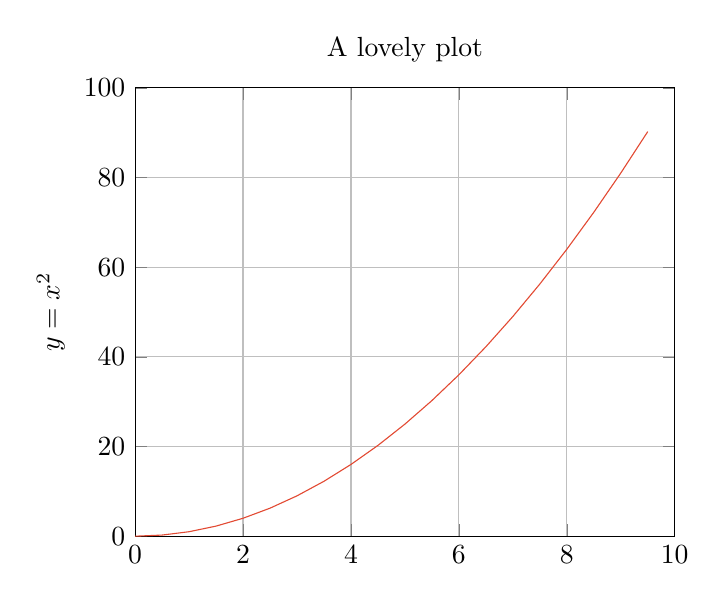
\begin{tikzpicture}

\definecolor{color0}{rgb}{0.886274509803922,0.290196078431373,0.2}

\begin{axis}[
title={A lovely plot},
ylabel={$y=x^2$},
xmin=0, xmax=10,
ymin=0, ymax=100,
xmajorgrids,
ymajorgrids
]
\addplot [color0]
coordinates {
(0,0)
(0.5,0.25)
(1,1)
(1.5,2.25)
(2,4)
(2.5,6.25)
(3,9)
(3.5,12.25)
(4,16)
(4.5,20.25)
(5,25)
(5.5,30.25)
(6,36)
(6.5,42.25)
(7,49)
(7.5,56.25)
(8,64)
(8.5,72.25)
(9,81)
(9.5,90.25)

};
\path [draw=white, fill opacity=0] (axis cs:13,0)--(axis cs:13,0);

\path [draw=white, fill opacity=0] (axis cs:13,1)--(axis cs:13,1);

\path [draw=white, fill opacity=0] (axis cs:0,13)--(axis cs:0,13);

\path [draw=white, fill opacity=0] (axis cs:1,13)--(axis cs:1,13);

\end{axis}

\end{tikzpicture}
  \end{figure}\vspace{5pt}
  \begin{figure}
       \setlength\figureheight{0.15\textheight}
    \setlength\figurewidth{0.4\textwidth}
    % This file was created by matplotlib v0.1.0.
% Copyright (c) 2010--2014, Nico Schlömer <nico.schloemer@gmail.com>
% All rights reserved.
% 
% The lastest updates can be retrieved from
% 
% https://github.com/nschloe/matplotlib2tikz
% 
% where you can also submit bug reports and leavecomments.
% 
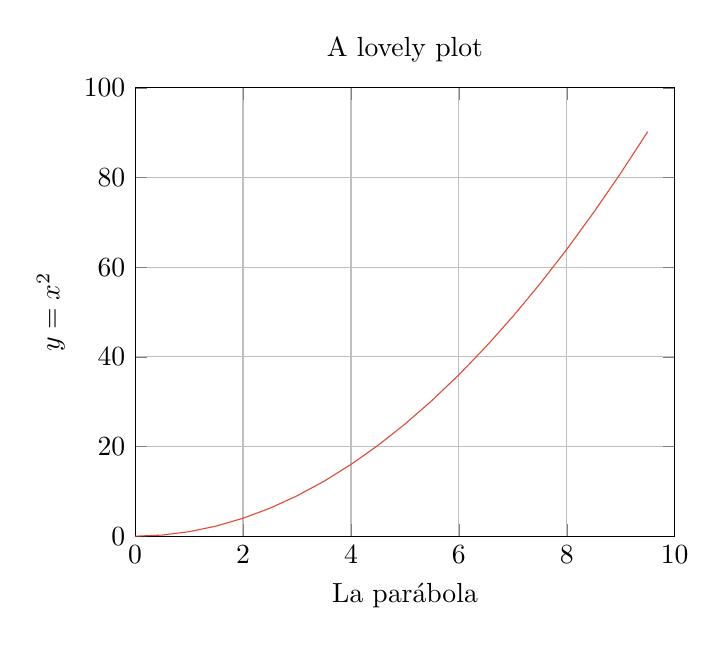
\begin{tikzpicture}

\definecolor{color0}{rgb}{0.886274509803922,0.290196078431373,0.2}

\begin{axis}[
title={A lovely plot},
xlabel={La parábola },
ylabel={$y=x^2$},
xmin=0, xmax=10,
ymin=0, ymax=100,
xmajorgrids,
ymajorgrids
]
\addplot [color0]
coordinates {
(0,0)
(0.5,0.25)
(1,1)
(1.5,2.25)
(2,4)
(2.5,6.25)
(3,9)
(3.5,12.25)
(4,16)
(4.5,20.25)
(5,25)
(5.5,30.25)
(6,36)
(6.5,42.25)
(7,49)
(7.5,56.25)
(8,64)
(8.5,72.25)
(9,81)
(9.5,90.25)

};
\path [draw=white, fill opacity=0] (axis cs:13,0)--(axis cs:13,0);

\path [draw=white, fill opacity=0] (axis cs:13,1)--(axis cs:13,1);

\path [draw=white, fill opacity=0] (axis cs:0,13)--(axis cs:0,13);

\path [draw=white, fill opacity=0] (axis cs:1,13)--(axis cs:1,13);

\end{axis}

\end{tikzpicture}
  \end{figure}\vspace{5pt}
  \begin{figure}
       \setlength\figureheight{0.05\textheight}
    \setlength\figurewidth{0.1\textwidth}
    % This file was created by matplotlib v0.1.0.
% Copyright (c) 2010--2014, Nico Schlömer <nico.schloemer@gmail.com>
% All rights reserved.
% 
% The lastest updates can be retrieved from
% 
% https://github.com/nschloe/matplotlib2tikz
% 
% where you can also submit bug reports and leavecomments.
% 
\begin{tikzpicture}

\begin{axis}[
title={A lovely plot},
xlabel={La parábola },
ylabel={$y=x^2$},
xmin=0, xmax=10,
ymin=0, ymax=100,
axis on top
]
\addplot [blue]
coordinates {
(0,0)
(0.5,0.25)
(1,1)
(1.5,2.25)
(2,4)
(2.5,6.25)
(3,9)
(3.5,12.25)
(4,16)
(4.5,20.25)
(5,25)
(5.5,30.25)
(6,36)
(6.5,42.25)
(7,49)
(7.5,56.25)
(8,64)
(8.5,72.25)
(9,81)
(9.5,90.25)

};
\path [draw=black, fill opacity=0] (axis cs:13,0)--(axis cs:13,0);

\path [draw=black, fill opacity=0] (axis cs:13,1)--(axis cs:13,1);

\path [draw=black, fill opacity=0] (axis cs:0,13)--(axis cs:0,13);

\path [draw=black, fill opacity=0] (axis cs:1,13)--(axis cs:1,13);

\end{axis}

\end{tikzpicture}
  \end{figure}\vspace{5pt}
  \begin{figure}
       \setlength\figureheight{0.25\textheight}
    \setlength\figurewidth{0.7\textwidth}
    % This file was created by matplotlib v0.1.0.
% Copyright (c) 2010--2014, Nico Schlömer <nico.schloemer@gmail.com>
% All rights reserved.
% 
% The lastest updates can be retrieved from
% 
% https://github.com/nschloe/matplotlib2tikz
% 
% where you can also submit bug reports and leavecomments.
% 
\begin{tikzpicture}

\begin{axis}[
title={A lovely plot},
xlabel={La parábola },
ylabel={$y=x^2$},
xmin=0, xmax=10,
ymin=0, ymax=100,
axis on top
]
\addplot [blue]
coordinates {
(0,0)
(0.5,0.25)
(1,1)
(1.5,2.25)
(2,4)
(2.5,6.25)
(3,9)
(3.5,12.25)
(4,16)
(4.5,20.25)
(5,25)
(5.5,30.25)
(6,36)
(6.5,42.25)
(7,49)
(7.5,56.25)
(8,64)
(8.5,72.25)
(9,81)
(9.5,90.25)

};
\path [draw=black, fill opacity=0] (axis cs:1,13)--(axis cs:1,13);

\path [draw=black, fill opacity=0] (axis cs:13,1)--(axis cs:13,1);

\path [draw=black, fill opacity=0] (axis cs:0,13)--(axis cs:0,13);

\path [draw=black, fill opacity=0] (axis cs:13,0)--(axis cs:13,0);

\end{axis}

\end{tikzpicture}
  \end{figure}\vspace{5pt}
  \begin{figure}
       \setlength\figureheight{0.25\textheight}
    \setlength\figurewidth{0.7\textwidth}
    % This file was created by matlab2tikz v0.6.0 running on MATLAB 7.14.
%Copyright (c) 2008--2014, Nico Schlömer <nico.schloemer@gmail.com>
%All rights reserved.
%Minimal pgfplots version: 1.3
%
%The latest updates can be retrieved from
%  http://www.mathworks.com/matlabcentral/fileexchange/22022-matlab2tikz
%where you can also make suggestions and rate matlab2tikz.
%
\begin{tikzpicture}

\begin{axis}[%
width=4.822222in,
height=3.803333in,
at={(0.808889in,0.513333in)},
scale only axis,
separate axis lines,
every outer x axis line/.append style={black},
every x tick label/.append style={font=\color{black}},
xmin=0,
xmax=10,
every outer y axis line/.append style={black},
every y tick label/.append style={font=\color{black}},
ymin=0,
ymax=100
]
\addplot[ycomb,color=blue,solid,mark=o,mark options={solid}] plot table[row sep=crcr] {%
0	0\\
1	1\\
2	4\\
3	9\\
4	16\\
5	25\\
6	36\\
7	49\\
8	64\\
9	81\\
10	100\\
};
\addplot [color=black,solid,forget plot]
  table[row sep=crcr]{%
0	0\\
10	0\\
};
\end{axis}
\end{tikzpicture}%
  \end{figure}\vspace{5pt}
  \begin{figure}
       \setlength\figureheight{0.25\textheight}
    \setlength\figurewidth{0.7\textwidth}
    % This file was created by matlab2tikz v0.6.0 running on MATLAB 7.14.
%Copyright (c) 2008--2014, Nico Schlömer <nico.schloemer@gmail.com>
%All rights reserved.
%Minimal pgfplots version: 1.3
%
%The latest updates can be retrieved from
%  http://www.mathworks.com/matlabcentral/fileexchange/22022-matlab2tikz
%where you can also make suggestions and rate matlab2tikz.
%
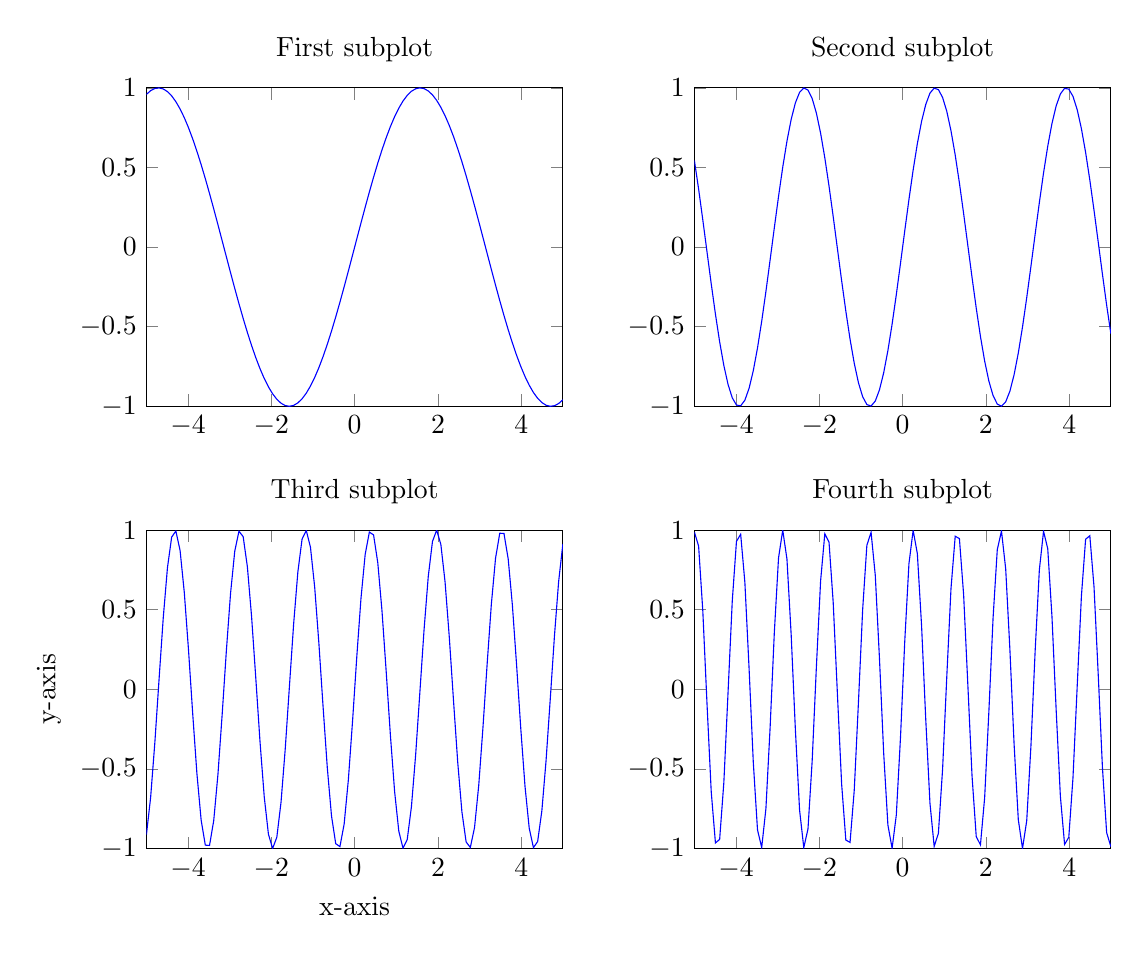
\begin{tikzpicture}

\begin{axis}[%
width=2.082323in,
height=1.592093in,
at={(3.548788in,0.513333in)},
scale only axis,
separate axis lines,
every outer x axis line/.append style={black},
every x tick label/.append style={font=\color{black}},
xmin=-5,
xmax=5,
every outer y axis line/.append style={black},
every y tick label/.append style={font=\color{black}},
ymin=-1,
ymax=1,
title={Fourth subplot}
]
\addplot [color=blue,solid,forget plot]
  table[row sep=crcr]{%
-5	0.988031624092862\\
-4.8989898989899	0.899928500486141\\
-4.7979797979798	0.491267969968986\\
-4.6969696969697	-0.0923837809243858\\
-4.5959595959596	-0.643128133910366\\
-4.49494949494949	-0.964788190970519\\
-4.39393939393939	-0.942787612159873\\
-4.29292929292929	-0.584963073936907\\
-4.19191919191919	-0.0187728199728824\\
-4.09090909090909	0.554104372439755\\
-3.98989898989899	0.92960781717014\\
-3.88888888888889	0.973981987569556\\
-3.78787878787879	0.671420662377814\\
-3.68686868686869	0.129697152232876\\
-3.58585858585859	-0.458224897886049\\
-3.48484848484848	-0.882925775468708\\
-3.38383838383838	-0.993125671111423\\
-3.28282828282828	-0.749571029926278\\
-3.18181818181818	-0.239016793197097\\
-3.08080808080808	0.356675988865319\\
-2.97979797979798	0.825319644206981\\
-2.87878787878788	0.999981805600717\\
-2.77777777777778	0.818447253157943\\
-2.67676767676768	0.345379174414414\\
-2.57575757575758	-0.25071406965208\\
-2.47474747474747	-0.757502161142318\\
-2.37373737373737	-0.994465562811467\\
-2.27272727272727	-0.877197153948598\\
-2.17171717171717	-0.447468316432701\\
-2.07070707070707	0.141650164941304\\
-1.96969696969697	0.680312405027813\\
-1.86868686868687	0.976645193022395\\
-1.76767676767677	0.925093843135269\\
-1.66666666666667	0.54402111088937\\
-1.56565656565657	-0.030833679061141\\
-1.46464646464646	-0.594705414024498\\
-1.36363636363636	-0.946741180583354\\
-1.26262626262626	-0.961544714026824\\
-1.16161616161616	-0.633842948448906\\
-1.06060606060606	-0.0803642996702817\\
-0.959595959595959	0.501740369393913\\
-0.858585858585859	0.905123515950136\\
-0.757575757575758	0.98609877449093\\
-0.656565656565657	0.71582249922919\\
-0.555555555555555	0.190567962875484\\
-0.454545454545454	-0.402567490669499\\
-0.353535353535354	-0.852307117939674\\
-0.252525252525253	-0.99845222690039\\
-0.151515151515151	-0.788945462844257\\
-0.0505050505050502	-0.298413804447639\\
0.0505050505050502	0.298413804447639\\
0.151515151515151	0.788945462844257\\
0.252525252525253	0.99845222690039\\
0.353535353535354	0.852307117939674\\
0.454545454545454	0.402567490669499\\
0.555555555555555	-0.190567962875484\\
0.656565656565657	-0.71582249922919\\
0.757575757575758	-0.98609877449093\\
0.858585858585859	-0.905123515950136\\
0.959595959595959	-0.501740369393913\\
1.06060606060606	0.0803642996702817\\
1.16161616161616	0.633842948448906\\
1.26262626262626	0.961544714026824\\
1.36363636363636	0.946741180583355\\
1.46464646464646	0.594705414024498\\
1.56565656565657	0.030833679061141\\
1.66666666666667	-0.544021110889371\\
1.76767676767677	-0.925093843135268\\
1.86868686868687	-0.976645193022395\\
1.96969696969697	-0.680312405027813\\
2.07070707070707	-0.1416501649413\\
2.17171717171717	0.447468316432703\\
2.27272727272727	0.877197153948597\\
2.37373737373737	0.994465562811467\\
2.47474747474747	0.757502161142318\\
2.57575757575758	0.250714069652077\\
2.67676767676768	-0.345379174414411\\
2.77777777777778	-0.818447253157943\\
2.87878787878788	-0.999981805600717\\
2.97979797979798	-0.825319644206979\\
3.08080808080808	-0.356675988865315\\
3.18181818181818	0.239016793197097\\
3.28282828282828	0.749571029926276\\
3.38383838383838	0.993125671111423\\
3.48484848484848	0.88292577546871\\
3.58585858585859	0.458224897886045\\
3.68686868686869	-0.129697152232876\\
3.78787878787879	-0.671420662377811\\
3.88888888888889	-0.973981987569557\\
3.98989898989899	-0.92960781717014\\
4.09090909090909	-0.554104372439753\\
4.19191919191919	0.0187728199728824\\
4.29292929292929	0.584963073936904\\
4.39393939393939	0.942787612159875\\
4.49494949494949	0.964788190970519\\
4.5959595959596	0.643128133910371\\
4.6969696969697	0.0923837809243858\\
4.7979797979798	-0.491267969968986\\
4.8989898989899	-0.899928500486144\\
5	-0.988031624092862\\
};
\end{axis}

\begin{axis}[%
width=2.082323in,
height=1.592093in,
at={(0.808889in,0.513333in)},
scale only axis,
separate axis lines,
every outer x axis line/.append style={black},
every x tick label/.append style={font=\color{black}},
xmin=-5,
xmax=5,
xlabel={x-axis},
every outer y axis line/.append style={black},
every y tick label/.append style={font=\color{black}},
ymin=-1,
ymax=1,
ylabel={y-axis},
title={Third subplot}
]
\addplot [color=blue,solid,forget plot]
  table[row sep=crcr]{%
-5	-0.912945250727628\\
-4.8989898989899	-0.679002966298063\\
-4.7979797979798	-0.335714142973882\\
-4.6969696969697	0.0616380370868729\\
-4.5959595959596	0.449064036623776\\
-4.49494949494949	0.764172829043648\\
-4.39393939393939	0.956219340264959\\
-4.29292929292929	0.99427642806427\\
-4.19191919191919	0.872215384559861\\
-4.09090909090909	0.609692902437243\\
-3.98989898989899	0.248985564019225\\
-3.88888888888889	-0.151818373399913\\
-3.78787878787879	-0.528173502056994\\
-3.68686868686869	-0.819471646794469\\
-3.58585858585859	-0.97880219676902\\
-3.48484848484848	-0.980506583396065\\
-3.38383838383838	-0.824310332501183\\
-3.28282828282828	-0.535367265601219\\
-3.18181818181818	-0.160208732147209\\
-3.08080808080808	0.240749792220685\\
-2.97979797979798	0.602938005079554\\
-2.87878787878788	0.868029169330635\\
-2.77777777777778	0.993333042454911\\
-2.67676767676768	0.958670706956729\\
-2.57575757575758	0.769624180301191\\
-2.47474747474747	0.456637487633774\\
-2.37373737373737	0.0701139604006468\\
-2.27272727272727	-0.327700708813498\\
-2.17171717171717	-0.672742503562265\\
-2.07070707070707	-0.909445943424462\\
-1.96969696969697	-0.999692340886112\\
-1.86868686868687	-0.928948429231251\\
-1.76767676767677	-0.708606797699218\\
-1.66666666666667	-0.374151230571219\\
-1.56565656565657	0.0205575962872592\\
-1.46464646464646	0.411955830830863\\
-1.36363636363636	0.737012758318913\\
-1.26262626262626	0.943381258446\\
-1.16161616161616	0.997827777979213\\
-1.06060606060606	0.89158425733514\\
-0.959595959595959	0.641760137619387\\
-0.858585858585859	0.288587058720434\\
-0.757575757575758	-0.111060038124129\\
-0.656565656565657	-0.492822042588923\\
-0.555555555555555	-0.79522005702305\\
-0.454545454545454	-0.969555949182324\\
-0.353535353535354	-0.987754692360084\\
-0.252525252525253	-0.846885563602984\\
-0.151515151515151	-0.569634106908965\\
-0.0505050505050502	-0.200648856522684\\
0.0505050505050502	0.200648856522684\\
0.151515151515151	0.569634106908965\\
0.252525252525253	0.846885563602984\\
0.353535353535354	0.987754692360084\\
0.454545454545454	0.969555949182324\\
0.555555555555555	0.79522005702305\\
0.656565656565657	0.492822042588923\\
0.757575757575758	0.111060038124129\\
0.858585858585859	-0.288587058720434\\
0.959595959595959	-0.641760137619387\\
1.06060606060606	-0.89158425733514\\
1.16161616161616	-0.997827777979213\\
1.26262626262626	-0.943381258445999\\
1.36363636363636	-0.737012758318914\\
1.46464646464646	-0.411955830830863\\
1.56565656565657	-0.0205575962872592\\
1.66666666666667	0.374151230571221\\
1.76767676767677	0.708606797699217\\
1.86868686868687	0.928948429231251\\
1.96969696969697	0.999692340886112\\
2.07070707070707	0.909445943424462\\
2.17171717171717	0.672742503562263\\
2.27272727272727	0.3277007088135\\
2.37373737373737	-0.0701139604006468\\
2.47474747474747	-0.456637487633774\\
2.57575757575758	-0.769624180301192\\
2.67676767676768	-0.958670706956729\\
2.77777777777778	-0.993333042454911\\
2.87878787878788	-0.868029169330635\\
2.97979797979798	-0.602938005079552\\
3.08080808080808	-0.240749792220684\\
3.18181818181818	0.160208732147209\\
3.28282828282828	0.535367265601216\\
3.38383838383838	0.824310332501183\\
3.48484848484848	0.980506583396065\\
3.58585858585859	0.978802196769019\\
3.68686868686869	0.819471646794469\\
3.78787878787879	0.528173502056997\\
3.88888888888889	0.151818373399911\\
3.98989898989899	-0.248985564019225\\
4.09090909090909	-0.609692902437246\\
4.19191919191919	-0.872215384559861\\
4.29292929292929	-0.99427642806427\\
4.39393939393939	-0.956219340264958\\
4.49494949494949	-0.764172829043648\\
4.5959595959596	-0.449064036623779\\
4.6969696969697	-0.0616380370868729\\
4.7979797979798	0.335714142973882\\
4.8989898989899	0.679002966298065\\
5	0.912945250727628\\
};
\end{axis}

\begin{axis}[%
width=2.082323in,
height=1.592093in,
at={(3.548788in,2.724574in)},
scale only axis,
separate axis lines,
every outer x axis line/.append style={black},
every x tick label/.append style={font=\color{black}},
xmin=-5,
xmax=5,
every outer y axis line/.append style={black},
every y tick label/.append style={font=\color{black}},
ymin=-1,
ymax=1,
title={Second subplot}
]
\addplot [color=blue,solid,forget plot]
  table[row sep=crcr]{%
-5	0.54402111088937\\
-4.8989898989899	0.364598733655889\\
-4.7979797979798	0.170346832328096\\
-4.6969696969697	-0.030833679061141\\
-4.5959595959596	-0.230760075325052\\
-4.49494949494949	-0.421300640588607\\
-4.39393939393939	-0.594705414024498\\
-4.29292929292929	-0.743921408256844\\
-4.19191919191919	-0.862879479381784\\
-4.09090909090909	-0.946741180583354\\
-3.98989898989899	-0.992095558932323\\
-3.88888888888889	-0.997097890943875\\
-3.78787878787879	-0.961544714026824\\
-3.68686868686869	-0.886882102029079\\
-3.58585858585859	-0.77614684828358\\
-3.48484848484848	-0.633842948448906\\
-3.38383838383838	-0.465758407025652\\
-3.28282828282828	-0.278729818677557\\
-3.18181818181818	-0.0803642996702817\\
-3.08080808080808	0.121269920537167\\
-2.97979797979798	0.317971662810619\\
-2.87878787878788	0.501740369393911\\
-2.77777777777778	0.665101514978822\\
-2.67676767676768	0.80141062216897\\
-2.57575757575758	0.905123515950137\\
-2.47474747474747	0.972021824958833\\
-2.37373737373737	0.999384557612436\\
-2.27272727272727	0.98609877449093\\
-2.17171717171717	0.932704855531834\\
-2.07070707070707	0.84137452086087\\
-1.96969696969697	0.71582249922919\\
-1.86868686868687	0.561155436815201\\
-1.76767676767677	0.383664191806112\\
-1.66666666666667	0.190567962875485\\
-1.56565656565657	-0.0102793412405343\\
-1.46464646464646	-0.210708548077193\\
-1.36363636363636	-0.402567490669496\\
-1.26262626262626	-0.578052585106573\\
-1.16161616161616	-0.730026229976446\\
-1.06060606060606	-0.852307117939675\\
-0.959595959595959	-0.939921651430131\\
-0.858585858585859	-0.98930623651434\\
-0.757575757575758	-0.99845222690039\\
-0.656565656565657	-0.9669876227093\\
-0.555555555555555	-0.896192201029956\\
-0.454545454545454	-0.788945462844257\\
-0.353535353535354	-0.649609513505707\\
-0.252525252525253	-0.483851640437935\\
-0.151515151515151	-0.298413804447641\\
-0.0505050505050502	-0.100838420258104\\
0.0505050505050502	0.100838420258104\\
0.151515151515151	0.298413804447641\\
0.252525252525253	0.483851640437935\\
0.353535353535354	0.649609513505707\\
0.454545454545454	0.788945462844257\\
0.555555555555555	0.896192201029956\\
0.656565656565657	0.9669876227093\\
0.757575757575758	0.99845222690039\\
0.858585858585859	0.98930623651434\\
0.959595959595959	0.939921651430131\\
1.06060606060606	0.852307117939675\\
1.16161616161616	0.730026229976446\\
1.26262626262626	0.578052585106572\\
1.36363636363636	0.402567490669497\\
1.46464646464646	0.210708548077193\\
1.56565656565657	0.0102793412405343\\
1.66666666666667	-0.190567962875486\\
1.76767676767677	-0.383664191806111\\
1.86868686868687	-0.561155436815201\\
1.96969696969697	-0.71582249922919\\
2.07070707070707	-0.841374520860871\\
2.17171717171717	-0.932704855531834\\
2.27272727272727	-0.98609877449093\\
2.37373737373737	-0.999384557612436\\
2.47474747474747	-0.972021824958833\\
2.57575757575758	-0.905123515950136\\
2.67676767676768	-0.80141062216897\\
2.77777777777778	-0.665101514978822\\
2.87878787878788	-0.501740369393911\\
2.97979797979798	-0.317971662810618\\
3.08080808080808	-0.121269920537166\\
3.18181818181818	0.0803642996702817\\
3.28282828282828	0.278729818677556\\
3.38383838383838	0.465758407025652\\
3.48484848484848	0.633842948448905\\
3.58585858585859	0.776146848283582\\
3.68686868686869	0.886882102029079\\
3.78787878787879	0.961544714026823\\
3.88888888888889	0.997097890943875\\
3.98989898989899	0.992095558932323\\
4.09090909090909	0.946741180583354\\
4.19191919191919	0.862879479381784\\
4.29292929292929	0.743921408256845\\
4.39393939393939	0.594705414024496\\
4.49494949494949	0.421300640588607\\
4.5959595959596	0.230760075325054\\
4.6969696969697	0.030833679061141\\
4.7979797979798	-0.170346832328096\\
4.8989898989899	-0.36459873365589\\
5	-0.54402111088937\\
};
\end{axis}

\begin{axis}[%
width=2.082323in,
height=1.592093in,
at={(0.808889in,2.724574in)},
scale only axis,
separate axis lines,
every outer x axis line/.append style={black},
every x tick label/.append style={font=\color{black}},
xmin=-5,
xmax=5,
every outer y axis line/.append style={black},
every y tick label/.append style={font=\color{black}},
ymin=-1,
ymax=1,
title={First subplot}
]
\addplot [color=blue,solid,forget plot]
  table[row sep=crcr]{%
-5	0.958924274663138\\
-4.8989898989899	0.982640507724898\\
-4.7979797979798	0.996339341557835\\
-4.6969696969697	0.999881125204762\\
-4.5959595959596	0.993229752418792\\
-4.49494949494949	0.976453029743715\\
-4.39393939393939	0.949721985269118\\
-4.29292929292929	0.913309125107055\\
-4.19191919191919	0.867585655364376\\
-4.09090909090909	0.813017697930967\\
-3.98989898989899	0.750161538661538\\
-3.88888888888889	0.679657956392746\\
-3.78787878787879	0.602225690607746\\
-3.68686868686869	0.518654114341195\\
-3.58585858585859	0.429795187019825\\
-3.48484848484848	0.336554769274278\\
-3.38383838383838	0.239883388262226\\
-3.28282828282828	0.140766547644453\\
-3.18181818181818	0.0402146809975962\\
-3.08080808080808	-0.0607471489178674\\
-2.97979797979798	-0.161089700024918\\
-2.87878787878788	-0.259790043402777\\
-2.77777777777778	-0.355841991401066\\
-2.67676767676768	-0.448266355087267\\
-2.57575757575758	-0.536120926459333\\
-2.47474747474747	-0.61851008366106\\
-2.37373737373737	-0.694593921281131\\
-2.27272727272727	-0.763596812658209\\
-2.17171717171717	-0.824815316904775\\
-2.07070707070707	-0.877625350042599\\
-1.96969696969697	-0.921488547144662\\
-1.86868686868687	-0.955957750625488\\
-1.76767676767677	-0.980681568730257\\
-1.66666666666667	-0.995407957751765\\
-1.56565656565657	-0.999986791456798\\
-1.46464646464646	-0.994371391528246\\
-1.36363636363636	-0.978619003421055\\
-1.26262626262626	-0.952890212780979\\
-1.16161616161616	-0.917447308375365\\
-1.06060606060606	-0.872651608224862\\
-0.959595959595959	-0.818959776194448\\
-0.858585858585859	-0.75691916659381\\
-0.757575757575758	-0.687162244245925\\
-0.656565656565657	-0.61040013690773\\
-0.555555555555555	-0.527415385771865\\
-0.454545454545454	-0.43905396795356\\
-0.353535353535354	-0.346216672288359\\
-0.252525252525253	-0.249849916358978\\
-0.151515151515151	-0.150936098365923\\
-0.0505050505050502	-0.0504835821984221\\
0.0505050505050502	0.0504835821984221\\
0.151515151515151	0.150936098365923\\
0.252525252525253	0.249849916358978\\
0.353535353535354	0.346216672288359\\
0.454545454545454	0.43905396795356\\
0.555555555555555	0.527415385771865\\
0.656565656565657	0.61040013690773\\
0.757575757575758	0.687162244245925\\
0.858585858585859	0.75691916659381\\
0.959595959595959	0.818959776194448\\
1.06060606060606	0.872651608224862\\
1.16161616161616	0.917447308375365\\
1.26262626262626	0.952890212780979\\
1.36363636363636	0.978619003421054\\
1.46464646464646	0.994371391528246\\
1.56565656565657	0.999986791456798\\
1.66666666666667	0.995407957751765\\
1.76767676767677	0.980681568730257\\
1.86868686868687	0.955957750625488\\
1.96969696969697	0.921488547144662\\
2.07070707070707	0.877625350042599\\
2.17171717171717	0.824815316904774\\
2.27272727272727	0.763596812658209\\
2.37373737373737	0.694593921281131\\
2.47474747474747	0.61851008366106\\
2.57575757575758	0.536120926459333\\
2.67676767676768	0.448266355087267\\
2.77777777777778	0.355841991401066\\
2.87878787878788	0.259790043402777\\
2.97979797979798	0.161089700024917\\
3.08080808080808	0.060747148917867\\
3.18181818181818	-0.0402146809975962\\
3.28282828282828	-0.140766547644452\\
3.38383838383838	-0.239883388262226\\
3.48484848484848	-0.336554769274278\\
3.58585858585859	-0.429795187019825\\
3.68686868686869	-0.518654114341195\\
3.78787878787879	-0.602225690607745\\
3.88888888888889	-0.679657956392747\\
3.98989898989899	-0.750161538661538\\
4.09090909090909	-0.813017697930967\\
4.19191919191919	-0.867585655364376\\
4.29292929292929	-0.913309125107055\\
4.39393939393939	-0.949721985269118\\
4.49494949494949	-0.976453029743715\\
4.5959595959596	-0.993229752418792\\
4.6969696969697	-0.999881125204762\\
4.7979797979798	-0.996339341557835\\
4.8989898989899	-0.982640507724898\\
5	-0.958924274663138\\
};
\end{axis}
\end{tikzpicture}%
  \end{figure}\vspace{5pt}
  \begin{figure}[H]
  \centering
       \setlength\figureheight{0.25\textheight}
    \setlength\figurewidth{0.7\textwidth}
    % This file was created by matplotlib v0.1.0.
% Copyright (c) 2010--2014, Nico Schlömer <nico.schloemer@gmail.com>
% All rights reserved.
% 
% The lastest updates can be retrieved from
% 
% https://github.com/nschloe/matplotlib2tikz
% 
% where you can also submit bug reports and leavecomments.
% 
\begin{tikzpicture}

\begin{axis}[
title={A lovely plot},
xlabel={La parábola },
ylabel={$y=x^2$},
xmin=0, xmax=10,
ymin=0, ymax=100,
axis on top
]
\addplot [blue]
coordinates {
(0,0)
(0.5,0.25)
(1,1)
(1.5,2.25)
(2,4)
(2.5,6.25)
(3,9)
(3.5,12.25)
(4,16)
(4.5,20.25)
(5,25)
(5.5,30.25)
(6,36)
(6.5,42.25)
(7,49)
(7.5,56.25)
(8,64)
(8.5,72.25)
(9,81)
(9.5,90.25)

};
\path [draw=black, fill opacity=0] (axis cs:1,13)--(axis cs:1,13);

\path [draw=black, fill opacity=0] (axis cs:13,1)--(axis cs:13,1);

\path [draw=black, fill opacity=0] (axis cs:0,13)--(axis cs:0,13);

\path [draw=black, fill opacity=0] (axis cs:13,0)--(axis cs:13,0);

\end{axis}

\end{tikzpicture}
    \caption{Esta figura est\'a en tikz}
  \end{figure}\vspace{5pt}
  \begin{figure}[H]
  \centering
  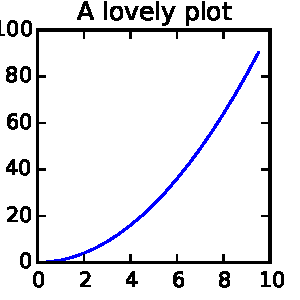
\includegraphics[scale=1]{figsize.pdf}
  \caption{Esta figura est\'a en pdf}
  \end{figure}
%   \begin{figure}[H]
%  \centering
%       \setlength\figureheight{0.25\textheight}
%    \setlength\figurewidth{0.7\textwidth}
%    \input{figsize1.tikz}
%    \caption{Esta figura est\'a en tikz}
%  \end{figure}\vspace{5pt}
  \begin{figure}[H]
  \centering
  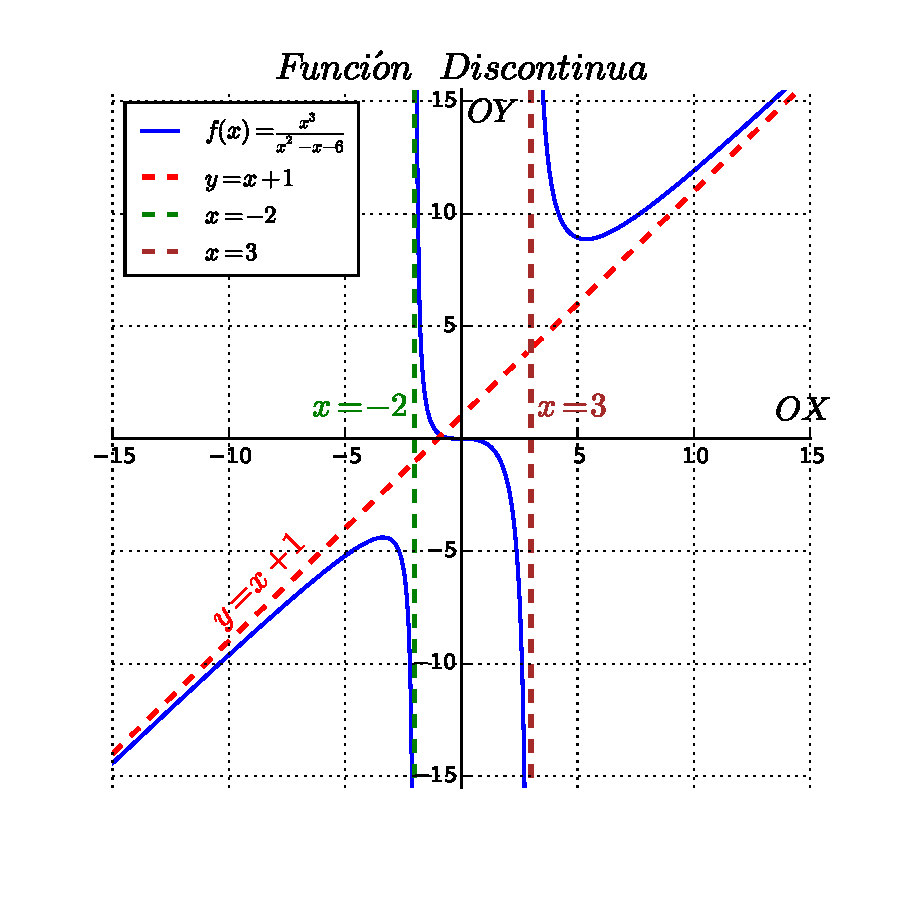
\includegraphics[scale=0.5]{figsize1.pdf}
  \caption{Esta figura est\'a en pdf}
  \end{figure}
   \begin{figure}[H]
  \centering
  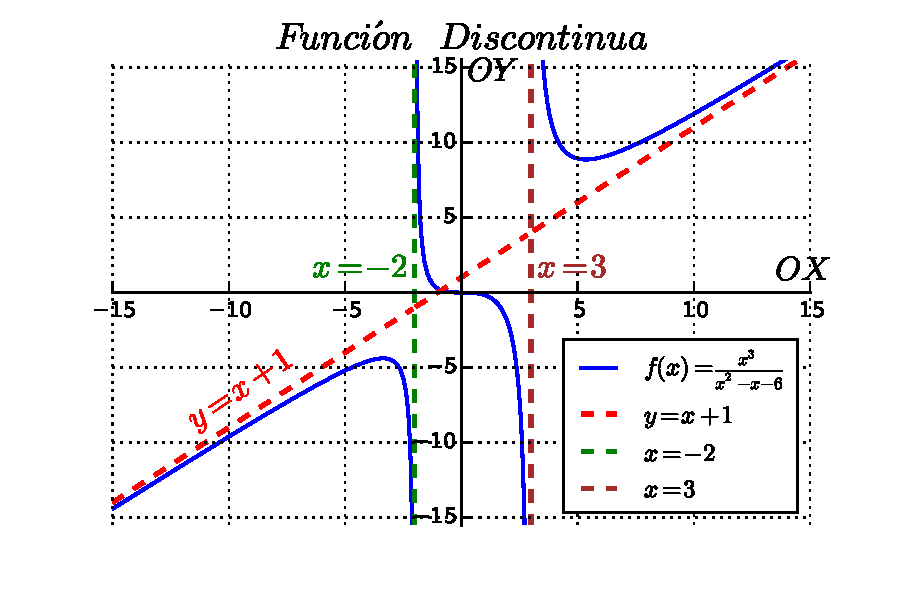
\includegraphics[scale=0.8]{figsize2.pdf}
  \caption{Esta figura est\'a en pdf escala 0.8}
  \end{figure}
   \begin{figure}[H]
  \centering
  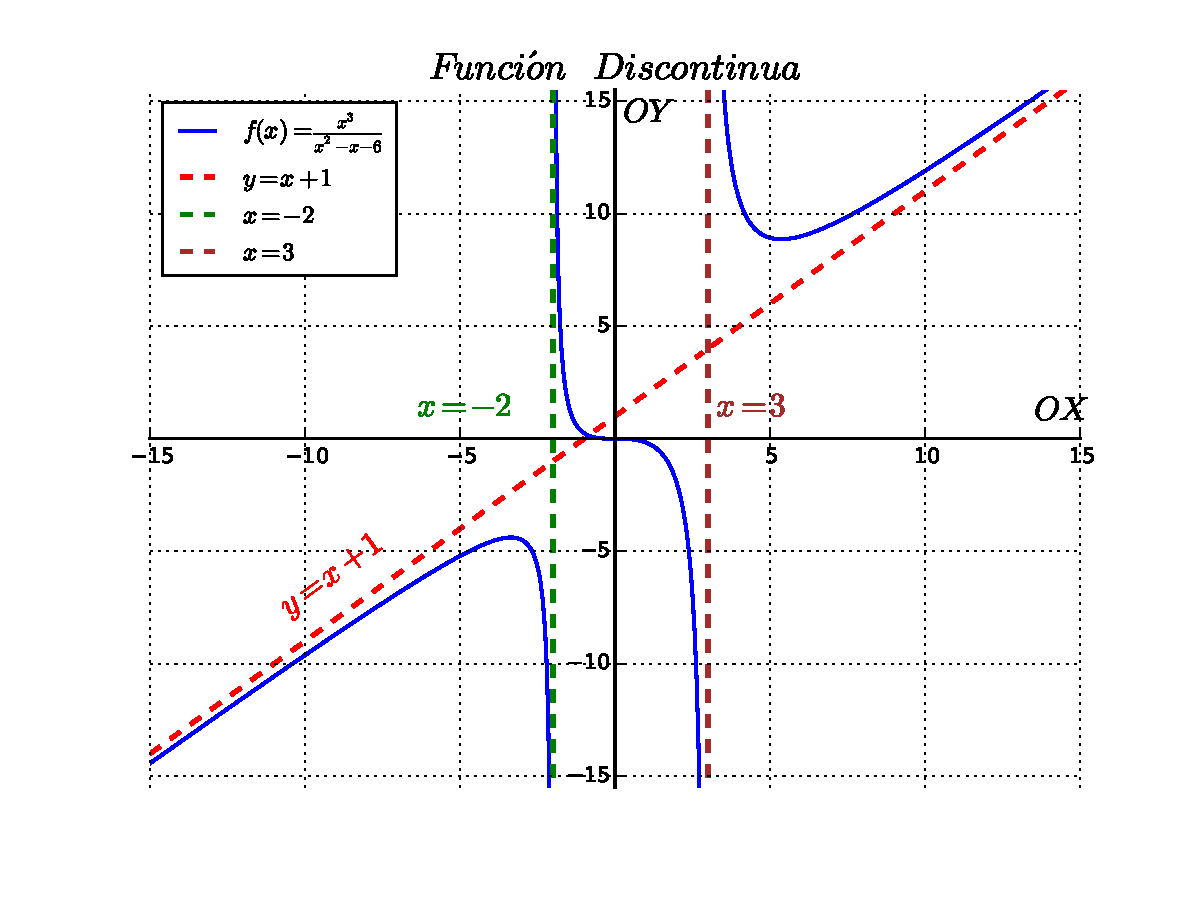
\includegraphics[scale=0.8]{figsize3.pdf}
  \caption{Esta figura est\'a en pdf escala 0.8}
  \end{figure}
  \begin{figure}[H]
  \centering
  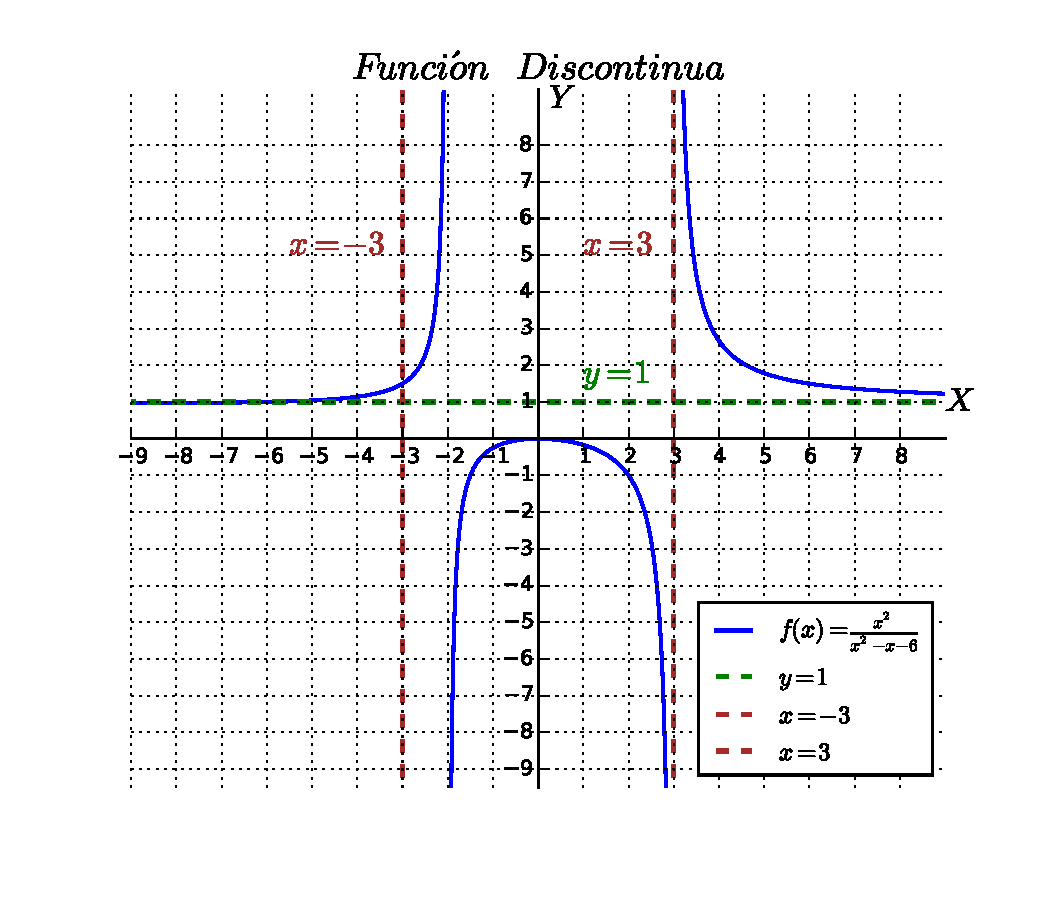
\includegraphics[scale=0.8]{figsize7.pdf}
  \caption{Esta figura est\'a en pdf escala 0.8}
  \end{figure}
  \begin{figure}[H]
  \centering
      %\documentclass[10pt]{article}
%\usepackage[T1]{fontenc}
%\usepackage{textcomp}
%
%\usepackage[utf8x]{inputenc}
%
%\usepackage{gnuplot-lua-tikz}
%\pagestyle{empty}
%\usepackage[active,tightpage]{preview}
%\PreviewEnvironment{tikzpicture}
%\setlength\PreviewBorder{2mm}
%
%
%\begin{document}

\begin{tikzpicture}[gnuplot]
%% generated with GNUPLOT 4.4p3 (Lua 5.1.4; terminal rev. 97, script rev. 96a)
%% dom 23 nov 2014 11:55:58 COT
\gpsolidlines
\gpcolor{gp lt color border}
\gpsetlinetype{gp lt border}
\gpsetlinewidth{1.00}
\draw[gp path] (1.196,0.616)--(1.376,0.616);
\draw[gp path] (12.147,0.616)--(11.967,0.616);
\node[gp node right] at (1.012,0.616) {-1};
\draw[gp path] (1.196,1.280)--(1.376,1.280);
\draw[gp path] (12.147,1.280)--(11.967,1.280);
\node[gp node right] at (1.012,1.280) {-0.8};
\draw[gp path] (1.196,1.943)--(1.376,1.943);
\draw[gp path] (12.147,1.943)--(11.967,1.943);
\node[gp node right] at (1.012,1.943) {-0.6};
\draw[gp path] (1.196,2.606)--(1.376,2.606);
\draw[gp path] (12.147,2.606)--(11.967,2.606);
\node[gp node right] at (1.012,2.606) {-0.4};
\draw[gp path] (1.196,3.270)--(1.376,3.270);
\draw[gp path] (12.147,3.270)--(11.967,3.270);
\node[gp node right] at (1.012,3.270) {-0.2};
\draw[gp path] (1.196,3.934)--(1.376,3.934);
\draw[gp path] (12.147,3.934)--(11.967,3.934);
\node[gp node right] at (1.012,3.934) { 0};
\draw[gp path] (1.196,4.597)--(1.376,4.597);
\draw[gp path] (12.147,4.597)--(11.967,4.597);
\node[gp node right] at (1.012,4.597) { 0.2};
\draw[gp path] (1.196,5.261)--(1.376,5.261);
\draw[gp path] (12.147,5.261)--(11.967,5.261);
\node[gp node right] at (1.012,5.261) { 0.4};
\draw[gp path] (1.196,5.924)--(1.376,5.924);
\draw[gp path] (12.147,5.924)--(11.967,5.924);
\node[gp node right] at (1.012,5.924) { 0.6};
\draw[gp path] (1.196,6.588)--(1.376,6.588);
\draw[gp path] (12.147,6.588)--(11.967,6.588);
\node[gp node right] at (1.012,6.588) { 0.8};
\draw[gp path] (1.196,7.251)--(1.376,7.251);
\draw[gp path] (12.147,7.251)--(11.967,7.251);
\node[gp node right] at (1.012,7.251) { 1};
\draw[gp path] (1.196,0.616)--(1.196,0.796);
\draw[gp path] (1.196,7.251)--(1.196,7.071);
\node[gp node center] at (1.196,0.308) { 0};
\draw[gp path] (2.939,0.616)--(2.939,0.796);
\draw[gp path] (2.939,7.251)--(2.939,7.071);
\node[gp node center] at (2.939,0.308) { 1};
\draw[gp path] (4.682,0.616)--(4.682,0.796);
\draw[gp path] (4.682,7.251)--(4.682,7.071);
\node[gp node center] at (4.682,0.308) { 2};
\draw[gp path] (6.425,0.616)--(6.425,0.796);
\draw[gp path] (6.425,7.251)--(6.425,7.071);
\node[gp node center] at (6.425,0.308) { 3};
\draw[gp path] (8.168,0.616)--(8.168,0.796);
\draw[gp path] (8.168,7.251)--(8.168,7.071);
\node[gp node center] at (8.168,0.308) { 4};
\draw[gp path] (9.911,0.616)--(9.911,0.796);
\draw[gp path] (9.911,7.251)--(9.911,7.071);
\node[gp node center] at (9.911,0.308) { 5};
\draw[gp path] (11.653,0.616)--(11.653,0.796);
\draw[gp path] (11.653,7.251)--(11.653,7.071);
\node[gp node center] at (11.653,0.308) { 6};
\draw[gp path] (1.196,7.251)--(1.196,0.616)--(12.147,0.616)--(12.147,7.251)--cycle;
\node[gp node right] at (10.679,6.917) {sin(x)};
\gpcolor{gp lt color 0}
\gpsetlinetype{gp lt plot 0}
\draw[gp path] (10.863,6.917)--(11.779,6.917);
\draw[gp path] (1.196,3.934)--(1.307,4.144)--(1.417,4.353)--(1.528,4.561)--(1.638,4.767)%
  --(1.749,4.969)--(1.860,5.166)--(1.970,5.359)--(2.081,5.546)--(2.192,5.727)--(2.302,5.900)%
  --(2.413,6.066)--(2.523,6.223)--(2.634,6.371)--(2.745,6.508)--(2.855,6.636)--(2.966,6.752)%
  --(3.076,6.858)--(3.187,6.951)--(3.298,7.033)--(3.408,7.101)--(3.519,7.157)--(3.630,7.201)%
  --(3.740,7.231)--(3.851,7.247)--(3.961,7.251)--(4.072,7.241)--(4.183,7.217)--(4.293,7.181)%
  --(4.404,7.131)--(4.514,7.069)--(4.625,6.993)--(4.736,6.906)--(4.846,6.807)--(4.957,6.696)%
  --(5.068,6.573)--(5.178,6.441)--(5.289,6.298)--(5.399,6.146)--(5.510,5.984)--(5.621,5.815)%
  --(5.731,5.638)--(5.842,5.454)--(5.952,5.264)--(6.063,5.068)--(6.174,4.868)--(6.284,4.664)%
  --(6.395,4.458)--(6.506,4.249)--(6.616,4.039)--(6.727,3.828)--(6.837,3.618)--(6.948,3.409)%
  --(7.059,3.203)--(7.169,2.999)--(7.280,2.799)--(7.391,2.603)--(7.501,2.413)--(7.612,2.229)%
  --(7.722,2.052)--(7.833,1.883)--(7.944,1.721)--(8.054,1.569)--(8.165,1.426)--(8.275,1.294)%
  --(8.386,1.171)--(8.497,1.060)--(8.607,0.961)--(8.718,0.874)--(8.829,0.798)--(8.939,0.736)%
  --(9.050,0.686)--(9.160,0.650)--(9.271,0.626)--(9.382,0.616)--(9.492,0.620)--(9.603,0.636)%
  --(9.713,0.666)--(9.824,0.710)--(9.935,0.766)--(10.045,0.834)--(10.156,0.916)--(10.267,1.009)%
  --(10.377,1.115)--(10.488,1.231)--(10.598,1.359)--(10.709,1.496)--(10.820,1.644)--(10.930,1.801)%
  --(11.041,1.967)--(11.151,2.140)--(11.262,2.321)--(11.373,2.508)--(11.483,2.701)--(11.594,2.898)%
  --(11.705,3.100)--(11.815,3.306)--(11.926,3.514)--(12.036,3.723)--(12.147,3.933);
\gpcolor{gp lt color border}
\gpsetlinetype{gp lt border}
\draw[gp path] (1.196,7.251)--(1.196,0.616)--(12.147,0.616)--(12.147,7.251)--cycle;
%% coordinates of the plot area
\gpdefrectangularnode{gp plot 1}{\pgfpoint{1.196cm}{0.616cm}}{\pgfpoint{12.147cm}{7.251cm}}
\end{tikzpicture}
%% gnuplot variables
%\end{document}

  \caption{Esta figura est\'a en set terminal tikz de gnuplot a una  escala 0.8}
  \end{figure}
  
  

\end{document}